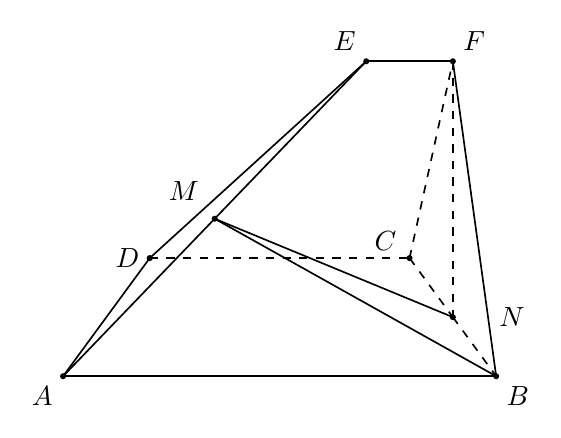
\begin{tikzpicture}[line width=0.6pt, scale=1.0, font=\normalsize]
  \coordinate (A) at (0,0);
  \coordinate (B) at (5.5000000000,0.0000000000);
  \coordinate (D) at (1.1,1.5);
  \coordinate (C) at (4.4000000000,1.5000000000);
  \coordinate (E) at (3.8500000000,4.0000000000);
  \coordinate (F) at (4.9500000000,4.0000000000);
  \coordinate (M) at (1.9250000000,2.0000000000);
  \coordinate (N) at (4.9500000000,0.7500000000);
  % solid visible edges
  \draw (A) -- (B);
  \draw (A) -- (D);
  \draw (A) -- (M);
  \draw (M) -- (E);
  \draw (D) -- (E);
  \draw (E) -- (F);
  \draw (F) -- (B);
  \draw (M) -- (N);
  % hidden edges
  \draw[dashed] (D) -- (C);
  \draw[dashed] (C) -- (F);
  \draw[dashed] (F) -- (N);
  \draw[dashed] (C) -- (N);
  \draw[dashed] (N) -- (B);
  \foreach \p in {A,B,C,D,E,F,M,N} {\fill (\p) circle (1.1pt);}
  \node[below left=2pt, , inner sep=1.5pt] at (A) {$A$};
  \node[below right=2pt, , inner sep=1.5pt] at (B) {$B$};
  \node[left=2pt, , inner sep=1.5pt] at (D) {$D$};
  \node[left=3pt,yshift=4pt,inner sep=1.5pt,xshift=0.000pt,yshift=2.008pt] at (C) {$C$};
  \node[above left=2pt, , inner sep=1.5pt] at (E) {$E$};
  \node[above right=2pt, , inner sep=1.5pt] at (F) {$F$};
  \node[left=4pt,yshift=10pt,inner sep=1.5pt] at (M) {$M$};
  \node[right=10pt,xshift=5pt,inner sep=1.5pt] at (N) {$N$};
\draw (M)--(B);
\end{tikzpicture}
